% ----------------------------------------------------
% Literature Review
% ----------------------------------------------------

\chapter{Literature Review}\label{ch:literature}

\section{Introduction}

This literature review starts with introducing the concept of salinity and its history.
It then discusses the importance and various uses of salinity measurements.
The review then covers the various documented methods of measuring salinity, followed by a review of the devices that used conductivity to measure salinity, which is the industry standard.
The review concludes with the theory and calculation of salinity from conductivity measurements.

\section{Salinity Definitions}\label{sec:a-brief-history-of-salinity}
The most commonly understood definition of salinity relates to the total amount of dissolved \textit{salts} in a solution. However, salinity's definition has had several more complex iterations over the last century.
One of the first definitions of salinity was the total amount of dissolved \textit{material} in grams in one kilogram of water~\cite{stewart_introduction_to_physical_oceanography_2004}, which is a dimensionless quantity that was expressed in \gls{ppt} or $g.kg^{-1}$ where most of the ocean water's salinity falls between 34.60\gls{ppt} and 34.80\gls{ppt}~\cite{stewart_introduction_to_physical_oceanography_2004}.

The problem with this definition lies in its testability.
Trying to obtain the mass of the dissolved material through evaporation removed certain compounds, making this method inaccurate~\cite{sverdrup_ocean_physics_and_chemistry_1942} and other methods of isolating the mass of the dissolved material had similar issues~\cite{stewart_introduction_to_physical_oceanography_2004}. 
The need for testability led to salinity being redefined in 1969 to be related to the amount of chlorine present in the water, better known as chlorinity~\cite{stewart_introduction_to_physical_oceanography_2004}.
Chlorinity measurements were well established, and the salinity calculation from chlorinity was relatively simple, which is further discussed in~\refsec{subsec:salinity-from-chlorinity}.

Around the same time as the salinity-chlorinity relationship was established, oceanographers began experimenting with using conductivity to measure salinity.
Conductivity was more precise and straightforward than the titration required to measure chlorinity~\cite{lewis_salinity_definition_and_calculation_1978}.
In 1978, the Practical Salinity Scale was established, which defined salinity in terms of conductivity and is regarded as the current definition of salinity~\cite{lewis_salinity_definition_and_calculation_1978}.
While the conductivity measurement was considered easy, the salinity-conductivity relationship was more complex as it had to include corrections for temperature and depth as they both affect the conductivity of an electrolyte solution~\cite{zheng_electrical_conductivity_of_ocean_2017}.

The Practical Salinity Scale uses dimensionless units of salinity, which are approximately equivalent to \glsreset{ppt}\gls{ppt}~\cite{seabird_ppt_vs_psu_2024} in the current definition of salinity~\cite{ioc_teos_2010}.
Although the Practical Salinity Scale is sometimes given in \gls{psu}, it is more technically correct to refer to it as a certain Practical Salinity `on the Practical Salinity Scale PSS-78'~\cite{lewis_salinity_definition_and_calculation_1978}.
The salinity calculation from conductivity is further discussed in~\refsec{sec:salinity-conductivity-relationship}.

\section{The Uses of Salinity Measurements}\label{sec:the-uses-of-salinity-measurements}
% oceanography, speciation, conservation, habitation, water quality (drinking, agriculture, industrial), aquaculture, desalination.
% antarctic ice.

\section{Salinity Measurement Methods}\label{sec:salinity-measurement-techniques}

Salinity has had a long history of being measured using various methods with varying degrees of accuracy.
Currently, the most common method of measuring salinity is using a \gls{ctd} instrument. 
However, there are multiple alternative methods, most of which have been developed over the last three decades, a summary of which is provided in \reftbl{tbl:salinity-measurement-methods}.

\begin{longtblr}[
    caption = {Summary of the various methods of measuring salinity.},
    label = {tbl:salinity-measurement-methods},
    ]{
    hlines,
    vlines,
    colspec = {Q[l,m,2.5cm]X[l,m]X[l,m]Q[l,m]}
    }
    \textbf{Method} & \textbf{Key Advantages} & \textbf{Key Disadvantages} & \textbf{Highest Accuracy} \\
    Chlorinity & {\textbullet~Concisely defined \\ \textbullet~Well established} & {\textbullet~Requires titration \\ \textbullet~Has human error} & 0.01\gls{ppt}~\cite{sverdrup_ocean_physics_and_chemistry_1942} \\
    Conductivity & {\textbullet~Industry standard \\ \textbullet~Automated devices available} & {\textbullet~Complex relationship \\ \textbullet~Requires temperature and depth corrections} & 0.0002~\gls{psu}~\cite{seabird_salinity_accuracy} \\
    Density & {\textbullet~Accounts for all dissolved material} & {\textbullet~Complex relationship \\ \textbullet~Requires temperature correction} & 0.003~\gls{psu}~\cite{millero_international_one_atmosphere_eos_seawater_1981} \\
    Microwave Radiation & {\textbullet~Measurable from a distance including from space} & {\textbullet~Requires many corrections \\ \textbullet~Expensive instrument} & 0.1~\gls{psu}~\cite{yueh_microwave_salinity_error_sources_2001} \\
    Refractive Index & {\textbullet~Compact devices available} & {\textbullet~Complex relationship \\ \textbullet~Requires temperature and pressure corrections} & 0.4\gls{ppt}~\cite{malarde_compact_refractometer_2008} \\
    Interferometry & {\textbullet~High accuracy reported} & {\textbullet~Large, complex instrument \\ \textbullet~Difficult to implement} & 0.001~\gls{psu}~\cite{yang_in_situ_refractometer_salinity_measurement_2024} \\
    Electromagnetic Induction & {\textbullet~Non-destructive} & {\textbullet~Not well researched \\ \textbullet~Large, high power instrument} & - \\
\end{longtblr}

\subsection{Salinity from Chlorinity}\label{subsec:salinity-from-chlorinity}

The chemical composition of ocean water with a salinity of 35\gls{ppt} contains 19.35\gls{ppt} of Chlorine and 10.77\gls{ppt} of Sodium with the following most common ions only accounting for just above 3\gls{ppt} of the total dissolved solids in the water~\cite{britannica_seawater_encyclopaedia_2024}.
This allowed oceanographers to determine that the salinity of ocean water was directly proportional to the amount of chlorine in the water, which holds true provided the ratios of the dissolved materials in the water remained constant.
The chlorinity of a solution has an established definition, which is `the mass of silver required to precipitate completely the halogens in $0.328\ 523\ 4 kg$ of the ocean-water sample'~\cite{wooster_redefinition_of_salinity_1969} which could be tested using titration.
In 1969, an accurate relationship between these was established by \refref{wooster_redefinition_of_salinity_1969}, shown in \refeqn{eqn:salinity-chlorinity}, which was significantly more accurate than the evaporation method achieving accuracies within 0.01\gls{ppt}~\cite{sverdrup_ocean_physics_and_chemistry_1942} but was still limited by human error~\cite{lewis_salinity_definition_and_calculation_1978}.
\begin{equation}\label{eqn:salinity-chlorinity}
 S (\text{\gls{ppt}}) = 1.80655 \times~Cl (\text{\gls{ppt}})
\end{equation}

\subsection{Salinity from Conductivity}\label{subsec:salinity-from-conductivity}

The conductivity of a liquid is a measure its ability to conduct electrical current, which is related to the number of free electrons present in the liquid, which is in turn related to the number of ions present in the liquid~\cite{stewart_introduction_to_physical_oceanography_2004}.
In the case of salt water, the ions present are from the dissolved material, which salinity was previously defined on~\cite{stewart_introduction_to_physical_oceanography_2004}.
The relationship between salinity and conductivity accounts for all the ions in the water as opposed to just chlorine which is why it was considered a more apt measure of salinity~\cite{lewis_salinity_definition_and_calculation_1978}.
Measuring conductivity was more accurate than titration, achieving accuracies within $0.0002$ on the Practical Salinity Scale PSS-78~\cite{seabird_salinity_accuracy}.
The conductivity measurement is typically done using a \gls{ctd} which measures the conductivity as well as the temperature and depth that are required to accurately calculate salinity.
\Gls{ctd} devices are discussed further in \refsec{sec:salinity-measurement-devices} and the calculation of salinity from conductivity is further discussed in~\refsec{sec:salinity-conductivity-relationship}.

\subsection{Salinity from Density}

The density of pure water varies with temperature and is approximately $1000 kg.m^{-3}$ at $4\degree C$~\cite{USGS_water_density_2018}.
Adding denser materials to the water will intuitively increase its density.
This concept is used to determine the quantity of added material using a density measurement, which can be used to calculate salinity~\cite{kjerfve_salinity_measurement_overview_1983}.
The relationship between salinity and density is approximately linear as shown in \refeqn{eqn:salinity-density} where $\rho$ is the density of the water, $\rho_0$ is the density of pure water, $k$ is a proportionality constant, and $S$ is the salinity of the water~\cite{uow_oceanography_research_1966}.
\begin{equation}\label{eqn:salinity-density}
    \rho = \rho_0(1 + kS)
\end{equation}
The more accurate relationship is more complicated and includes a temperature correction defined by \refref{millero_international_one_atmosphere_eos_seawater_1981}.
While the accuracy of salinity from density was less than that from conductivity with accuracies within $0.003$ on the Practical Salinity Scale PSS-78~\cite{millero_international_one_atmosphere_eos_seawater_1981}, \refref{schmidt_density_salinity_relation_2018} still claimed that density was more appropriate to use as the standard potassium chloride solution used to calibrate the \glspl{ctd} meters did not account for the variation of the ratios of conductive and non-conductive materials commonly present in salt water while the density of the water did.

\subsection{Salinity from Microwave Radiation}

The electromagnetic spectrum interacts uniquely with salt water, scattering, refracting, and reflecting when in contact with it or any material dissolved in it.
Different temperature molecules in the water interact with electromagnetic waves differently, and the pressure of the water also varies this interaction. However, the most significant effect is from the presence of the dissolved material~\cite{swift_considerations_for_microwave_salinity_1983}.

Microwave radiation is one section of the electromagnetic spectrum that takes advantage of this fact to measure salinity~\cite{swift_considerations_for_microwave_salinity_1983}.
Microwave radiation does not require direct contact with the water to make a measurement, making it possible to measure the salinity of a water sample from a far distance, including from space~\cite{gabarro_microwave_salinity_2004}.
This necessitated the investigation of the relationship that could accurately predict salinity from a microwave reading~\cite{gabarro_microwave_salinity_2004}.
The relationship required multiple different corrections as the microwave readings were found to be affected by \gls{sst}, surface air pressure, surface air temperature, faraday rotation, and surface wind speed~\cite{yueh_microwave_salinity_error_sources_2001}.

This research has allowed for the development of satellites that can measure the salinity, which has been used to develop global salinity maps as shown in \reffig{fig:satellite_salinity_map}.
The data measured using this method is reported to be accurate to within $0.1$ on the Practical Salinity Scale PSS-78~\cite{yueh_microwave_salinity_error_sources_2001}.
\begin{figure}[ht]
    \centering
    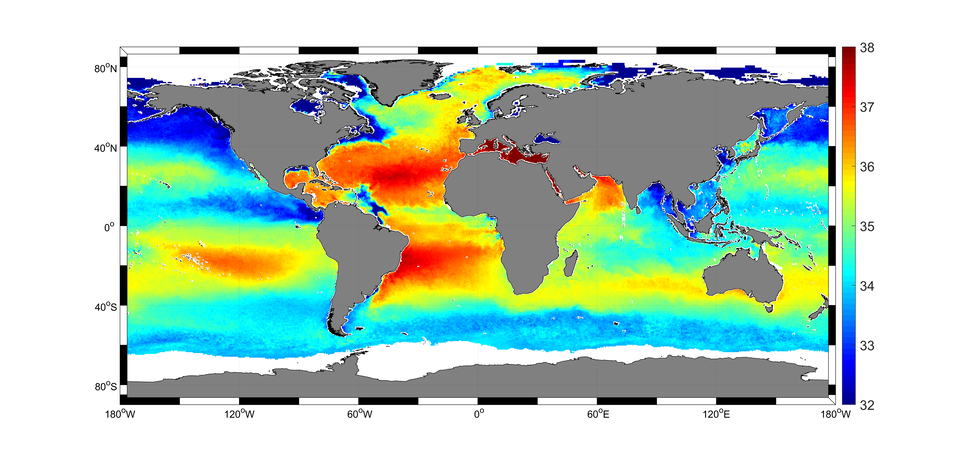
\includegraphics[width=0.75\textwidth]{Figures/salinity_distribution}
    \caption{Global salinity map generated using satellite data~\cite{esa_mapping_salty_waters_2019}.}
    \label{fig:satellite_salinity_map} %chktex 24
\end{figure}

\subsection{Salinity from Refractive Index}

The second measurement method that takes advantage of the electromagnetic spectrum interaction uses the visible light spectrum to measure the water's refractive index.
The relationship between salinity and refractive index is similarly complex, requiring a 27-term equation that includes the effect of pressure and temperature.
The refractive index equation is defined a range of $500-700nm$ in wave length, $0-30\degree C$ in temperature, $0-40$ on the Practical Salinity Scale PSS-78, and $0-11000 dbar$ in pressure, and it holds an accuracy of $0.4-80$ \gls{ppm} on the Practical Salinity Scale PSS-78, decreasing with increasing pressure.~\cite{millard_index_of_refraction_algorithm_1990}

Refractometers are used to measures the refractive index of water and as only a small amount of the sample is needed, these devices are relatively compact.
Two notably compact versions have dimensions of $22.5mm \times 22.5mm \times 120mm$~\cite{malarde_compact_refractometer_2008} and $40mm \times 40mm \times 70mm$~\cite{tengesdal_compact_refractometer_2012} which have achieved accuracies of 2 and 83 \gls{ppt} on the Practical Salinity Scale PSS-78 respectively.

\subsection{Salinity from Interferometry}

The last measurement method that uses the electromagnetic spectrum is interferometry.
Interferometry involves generating two identical light waves on the visible spectrum, passing one through the sample and the other through a non-interfering medium, and then comparing the two waves.
The comparative gain and phase shift between the two waves can be used to identify the salinity of a sample of salt water~\cite{liao_interferometer_seawater_salinity_2023}.

This method has varying implementations, each with varying results.
\refref{yang_in_situ_refractometer_salinity_measurement_2024} reported to be accurate within $0.001$ on the Practical Salinity Scale PSS-78 using a Michelson interferometer and other researchers have reported other accuracies using different interferometers~\cite{possetti_interferometer_salinity_measurement_2009, nguyen_interferometer_salinity_measurement_2009, zhao_interferometer_salinity_measurement_2009}.
The refractometer has the disadvantage of being a large instrument requiring precisely aligned and spaced mirrors to direct the light waves, making it difficult to implement in a compact device. 

\subsection{Salinity from Magnetic Permeability}\label{subsec:salinity-from-electromagnetic-induction}

Similarly to conductivity, a liquid's magnetic permeability is related to the number of ions present in it.
The more ions present in the liquid, the stronger the magnetic alignment that the liquid can generate, increasing its magnetic permeability.
In salt water, this is related to the total dissolved solids~\cite{somaraju_electromagnetic_salinity_2006}.

Several methods are available for measuring a liquid's magnetic permeability, including \gls{lcr} meters~\cite{waltrip_inductance_measurement_2005}, resonant circuits~\cite{alhassoon_complex_permittivity_extraction_2021}, magnetic force sensors~\cite{pattakos_magnetic_permeability_sensor_2023}, and a permeability bridge~\cite{ewing_magnetic_balance_permeability_1898}.
These methods all have the advantage of not requiring direct contact with the salt water to make a measurement, which allows for the sample to remain undisturbed, unlike conductivity and other methods which may be destructive~\cite{tengesdal_electromagnetic_salinity_2014}.
While the measurement of the magnetic permeability is well-defined, the relationship between it and salinity has yet to be thoroughly investigated.
Additionally, the equipment required to measure the magnetic permeability is relatively large and typically has a high power consumption, making it difficult to compact for use in remote environments.

\section{Salinity Measurement Devices using Conductivity}\label{sec:salinity-measurement-devices}

There are several commercial \gls{ctd} devices available from small handheld devices such as the \href{https://euca.co.za/products/salinity-pen?srsltid=AfmBOorAK21_xoeOZbaqoqXbRzrLxF5Yx47nzn7tvsve-_Azl3sSh1-QbIg}{Salinity Pen} to large oceanographic research devices such as \href{https://oceanexplorer.noaa.gov/technology/ctd/ctd.html}{Ocean Exploration's CTD}.
These devices are used in various applications with varying prices and accuracies. 
The fundamental concept of the device involves placing two electrodes in a sample of water, applying a voltage across them, and measuring the water's response.
This is paired with a temperature and depth correction, which allows a salinity value to be calculated, which is discussed in \refsec{sec:salinity-conductivity-relationship}.
Unfortunately, most of \gls{ctd}'s technology is proprietary so the exact workings of their devices are not published.

Some researchers have developed their own \gls{ctd} devices for specific applications.
A study investigating the effect of human activities that alter the salt concentration of water sources such as lakes, ponds and wetlands in Illinois, USA, developed their own \gls{ctd}.
The device reported an average error of 6\% in the laboratory validation and 11\% in the field validation.
It used an alternative approximation of converting the conductivity to salinity, which used single voltage readings to measure the resistance of the water samples, which were then used to create a sensor-specific mathematical model to convert the resistance to salinity~\cite{benjankar_ec_based_salt_measurement_2021}.
A similar device was shown on a forum with a similar design principle; however, this one was significantly less advanced, making no attempt to correlate the measured resistance values to a salinity value~\cite{instructables_water_salinity_meter}.

Researchers at Uppsala University in Sweden developed a nano \gls{ctd} probe that measured $7.5 \times 3.5mm$ in size, shown in \reffig{fig:nano-ctd}.
The probe contained everything required for an accurate salinity measurement, and each of the sensors achieved a high degree of accuracy.
The probe achieved a high $r^2$ value of $0.9787$ and a standard deviation of 2.37\gls{ppt} using an alternating current at 42kHz to measure the conductivity.
This design indicated that miniaturized salinometers are viable and could be used in devices such as bio-loggers on marine animals.~\cite{jonsson_chip_based_salinity_2013}
\begin{figure}[ht]
    \centering
    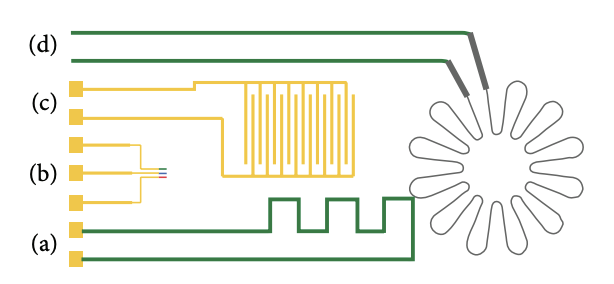
\includegraphics[width=0.75\textwidth]{Figures/nano_ctd}
    \caption{The schematic of a \gls{ctd} probe developed by researchers at Uppsala University in Sweden which design contains (a) a temperature sensor, (b) three relatively small electrodes for pH and Cl- concentration, (c) conductivity electrodes, and (d) a strain gauge for the pressure membrane sensor. The design is $7.5 \times 3.5 mm$ in size~\cite{jonsson_chip_based_salinity_2013}.}
    \label{fig:nano-ctd} %chktex 24
\end{figure}

% CTDs, refractometers, conductivity meters, salinometers.

% ----------------------------------------------------
%current CTDs
%
%electrical conductivity sensor https://link.springer.com/article/10.1007/s11270-020-04971-7
%
%arduino version https://www.instructables.com/Water-Salinity-meter/
%
%mini version https://www.diva-portal.org/smash/get/diva2:512332/FULLTEXT01.pdf
%
%% ----------------------------------------------------
%measurement techniques
%
%high res https://link.springer.com/chapter/10.1007/978-1-4615-9182-5_18
%
%salinity and its measurands https://iopscience.iop.org/article/10.1088/1681-7575/aaea92/pdf
%
%interferometer https://iopscience.iop.org/article/10.1088/0957-0233/20/3/034003/meta?casa_token=ZTZbYNUpO0kAAAAA:7jvq44f2kE5qGGEQWt5ji18A7xWG4p9ZT4Ny99eOjMPOfywPIgqRNoCeH0VZby1VjlART_v77WV3rxfwi0k1nwphxfguYA
%
%the whole suite, important for later https://www.researchgate.net/profile/Bjoern-Kjerfve/publication/255660361_Measurement_and_Analysis_of_Water_Current_Temperature_Salinity_and_Density/links/0c9605373c5d3088b4000000/Measurement-and-Analysis-of-Water-Current-Temperature-Salinity-and-Density.pdf
%
%microwave frequency https://www.sensorsportal.com/HTML/DIGEST/january_2014/Vol_162/P_1772.pdf
%
%refraction of light https://www.sciencedirect.com/science/article/abs/pii/S0925400503002922?casa_token=UDq5jm83UIsAAAAA:-UuQMhyBg9tuzleSc8tQnL2vuCv_HYHCB5AicHCTlBkBz_5gipNnDoA6DdPgBL9csU_wWS9lG6Bc
%
%conductivity using electromagnetism https://ieeexplore.ieee.org/abstract/document/7769877
%
%salinity equation paper https://agupubs.onlinelibrary.wiley.com/doi/abs/10.1029/jc083ic01p00466?casa_token=Om_oxKhUgLIAAAAA%3As_ZdT6Qn-zv9SSyC8G3io5r_0mxuepRxFE33jcaLtTNY4tyOQOLAObVtsjeQZ0gPpokwsmrEOP0pPHULQg
%
%% ----------------------------------------------------
%salinity properties
%
%temperature vs salinity https://link.springer.com/article/10.1023/B:EMAS.0000031719.83065.68
%
%salinity and other properties https://pubs.acs.org/doi/10.1021/es402188r
%
%salinity and it antecedents https://ieeexplore.ieee.org/stamp/stamp.jsp?tp=&arnumber=1145448
%
%salinity textbook https://pubs.acs.org/doi/pdf/10.1021/ja02205a013?casa_token=QPyPLh22vacAAAAA:O6Hc1M5FQEDZpJb4oUrGYzboIy0wWn__w6MxXGc8Aw7doPE9tz71yRCbmUtRSP5lOMdTr28U8bYI43IsBg
%
%electrical properties of salt ice https://pubs.acs.org/doi/full/10.1021/jp8055366?casa_token=qvssn_P9p_8AAAAA%3A1FY_4CW5oX_4P9gDNZfp0AaeByCkTF_WOcZ_hLbv2Y2FYsIRsO7ZZkqxzTHTo_MK4vWqfaqqQh2LagyDLA
%
%pressure and temperature increase conductivity https://journals.aps.org/pr/abstract/10.1103/PhysRev.70.329
%
%conductivity vs total dissolved solids https://iopscience.iop.org/article/10.1088/1755-1315/118/1/012019/meta
%
%% ----------------------------------------------------
%producers or CTDs
%
%https://www.whoi.edu/what-we-do/explore/instruments/instruments-sensors-samplers/conductivity-temperature-depth-ctd-sensors/
%
%% ----------------------------------------------------

